\documentclass[letterpaper,titlepage,spanish,10pt]{article}
\usepackage[latin1]{inputenc}    % Agregar y acentos
\usepackage{babel}               % Soporte multilenguajes
\usepackage{avant}               % Tipo de fuente
%\usepackage{fancyheadings}      % Topes y pies de p'agina
\usepackage[dvips]{graphicx}     % Inclusion de imagenes .eps
\usepackage{url}                 % Agregar Links soporte de ~
\usepackage{verbatim}
\usepackage{geometry}
\usepackage{url}
\usepackage{amsfonts}
\usepackage{amssymb}
%\usepackage{txfonts}
%\usepackage{emphoff}
%\usepackage{pxfonts}
%\usepackage{fancybox}
\usepackage{latexsym}
%\usepackage{fancyvrb}
\usepackage{graphicx}
%\usepackage{wasysym}
%\renewcommand{\baselinestretch}{1.5}
\parskip=7mm
\pagestyle{myheadings}
\geometry{tmargin=4cm, bmargin=4cm, lmargin=2.5cm, rmargin=2.5cm}
\markright{\hrulefill Plan de Negocio - Software Hevelius $\; \;$}


%opening
\title{{\Huge \bf Plan de Negocio} \\ {\Large Software Hevelius} \\ {\small Empresa DevNull}}

\author{
{\bf Carlos Guajardo Miranda} \\ \url{cguajard@alumnos.inf.utfsm.cl}
\and
{\bf Marina Pilar Daza} \\ \url{mpilar@alumnos.inf.utfsm.cl}
\and
{\bf Esteban Espinoza Mart\'inez} \\ \url{eespinoz@alumnos.inf.utfsm.cl}
\and
{\bf Tom\'as Staig Fern\'andez} \\ \url{tstaig@alumnos.inf.utfsm.cl}
}


\date{11 de octubre de 2007}


\begin{document}

% Portada
\maketitle
\newpage

% Indices
\tableofcontents{}
\newpage

\section{Resumen Ejecutivo}
%Descripci�n: Documento de presentaci�n que motiva a leer el resto del documento por el inter�s que despierta.
Nuestra Empresa se desarrolla en el \'area inform\'atica y cient\'ifica generando software que facilita
el trabajo de investigaci\'o. Ante este principio, estamos desarrollando un software que permite el control
de cualquier telescopio bajo la misma interfaz.

Durante los dos semestres disponibles para el desarrollo del proyecto Hevelius, pretendemos dise\~nar y desarrollar 
un sistema de control de telescopios, el cual tiene como caracter\'istica principal el car\'acter gen\'erico.
En la actualidad cada software para controlar telescopios es de car\'acter individual, vale decir, 
existe una determinada interfaz y sistema de control espec\'ifico para cada distinto telescopio, 
transformando as\'i la tarea de los operadores de \'estos un trabajo tedioso, puesto que deben aprender 
a utilizar distintas interfaces y sistemas para cada uno de los instrumentos.
Esta propuesta, como se mencion\'o anteriormente, pretende eliminar esta complicaci\'on y hacer m\'as 
sencilla la tarea de los operadores, esto mediante una interfaz gen\'erica que permita ser aplicable 
a cada telescopio sin importar el tipo de \'este, con lo cual los operadores ya no tendr\'an que 
aprender dos o m\'as tipos de interfaces y sistemas, si no que bastar\'a s\'olo con una.
Otro car\'acter importante de nuestro proyecto es la implementaci\'on de algoritmos de tracking,
 lo cual permite compensar el movimiento de la tierra en la observaci\'on de alg\'un objeto espacial 
(estrella, cometa, etc.) sin intervenir el software, esto debido a la implementaci\'on de un control autom\'atico,
 el cual permitir\'a la ausencia de un operador en esta tarea. Este control autom\'atico ser\'a capaz de detectar
 posiciones y coordenas que puedan da\~nar al telescopio. Todo esto ayuda no s\'olo los operadores de telescopios, 
si no que a los mismos astr\'onomos, obteniendo una mayor cantidad de datos para analizar, adem\'as de los importantes
 controles sobre la luminosidad lunar, con el fin de evitar da\~nos al equipamiento.
Hevelius pretende ser un sistema de alta disponibilidad, esto implica que ante una eventual ca\'ida en una estaci\'on conectada a un telescopio,
 el sistema se puede emplear desde otra estaci\'on, sin p\'erdida de datos y permitiendo el r\'apido reinicio de las actividades.
En conclusi\'on, nuestro proyecto busca desarrollar una herramienta para usuarios profesionales en el \'area del control de telescopios,
 teniendo \'esta como mayor caracter\'istica la generalidad. Otro punto que cabe destacar, es el hecho de que el proyecto Hevelius 
se inserta en otro proyecto de nivel internacional, por lo que toda la documentaci\'on debe ser escrita en el idioma Ingl\'es, 
con el objetivo de no solo hacer un aporte a nivel global, si no que tambi\'en que sirva como incentivo a futuros grupos que deseen 
continuar mejorando y/o realizando proyectos que tengan este car\'acter gen\'erico para un \'ambito tan complejo como es el manejo
 de estos instrumentos llamados telescopios.





\newpage
\section{El Producto: \textit{Hevelius}}
%    *  Presentaci�n breve pero completa del producto
Hevelius es un software dedicado al control de diversos telescopios a trav\.es de una interfaz gr\.afica, mediante la cual se quiere dar los primeros pasos para un control gen\.erico de telescopios con flexibilidad en su estructura como software, es decir, que se pueda ser reconocido por cualquier telescopio.
Hevelius esta dise\~nado principalmente para un manejo a nivel profesional de telescopio, para ello esta compuesto por una serie de componentes para cumplir con estos requerimientos como son:
\begin{itemize}
\item Telescopio a escala que muestra la ubicaci\.on actual en que se encuentra el telescopio.
\item Imagen de lo que actualmente esta observando el telescopio. 
\item Control de accesibilidad de lo que se quiera observar
\item Presetting, capacidad de moverse desde cierta ubicaci\.on a otra de manera segura
\item Tracking, capacidad del telescopio de seguir cierto objeto en el cielo, contrarrestando el movimiento de la Tierra.
\item Poiting Manual, capacidad del telescopio de seguir cierto objeto en el cielo, contrarrestando el movimiento de la Tierra.
\item Catalogo de Estrellas para observaci\.on directa de estrellas conocidas
\item Limitantes que puedan da\~nar el telescopio, como la luz directa de la luna
\item Informaci\.on detallada del clima que se vive actualmente en el lugar donde se encuentra el telescopio.
\item Bot\.on de emergencia para detener la observaci\.on inmediatamente por posibles problemas u errores de observaci\.on.
\end{itemize}
Una visi\.on de c\.omo se encuentra actualmente Hevelius es la siguiente:
\begin{figure}[h!]
 \centering
 \includegraphics[scale=0.5]{hevelius1.eps}
 \caption{Interfaz de un telescopio}
 %\label{fig:yeti}
\end{figure}

\begin{figure}[h!]
 \centering
 \includegraphics[scale=0.5]{hevelius2.eps}
 \caption{Interfaz de un telescopio}
 %\label{fig:yeti}
\end{figure}

%    * �Qu� problema soluciona?
Controlar un telescopio no es una tarea f\.acil, ya que no basta con encontrar una adecuada ubicaci\.on para que sea m\.as propicia la observaci\.on, sino que tambi\.en son instrumentos que requieren un estudio previo antes de ser usados con la finalidad de no da\~narlos, sin contar que cada tipo de telescopio tiene una manera distinta de operarlo. De acuerdo a su dise\~nador o lugar en que fue creado, var\.ia la forma en que est\.a implementada, lo que hace que tanto los astr\.onomos como gente aficionada que trabaja con estos instrumentos tiene que implementar gran parte de su tiempo en aprender como trabajar con cada equipo de adquieren, lo que hace la tarea m\.as engorrosa a medida que se tienen m\.as equipos, ya que no hay una forma eficiente para evitar utilizar interfaces distintas para cada telescopio lo que se convierte en un problema.

Adem\.as existe el problema de que no existe una interfaz que pueda direccionar el telescopio de acuerdo a coordenadas que el operador de telescopio pueda ingresar o, a la vez, consultar la ubicaci\.on de alg\.un cuerpo. Tampoco existe alguna interfaz amigable para el operador de telescopio, ya que en la actualidad, estas son muy engorrosas y poco claras para el uso r\.apido y eficaz, considerando aspectos tan importantes como la luminosidad de la Luna con tal de prevenir da\~nos en los equipos.

Es por eso imperante la necesidad de crear un software que sea capaz de cumplir con los puntos mencionados anteriormente, permitiendo que el manejo de los telescopios quede en forma gen\.erica y sea capaz de prevenir un posible da\~no por coordenadas que puedan estar muy cerca de la luna.

%    * �A qu� cliente responde y c�mo es el tipo de usuario?
Actualmente .Software development for ALMA-CONICYT: Building up expertise to meet ALMA-CONICYT software requirements within a Chilean University., es un proyecto en desarrollo en la Universidad T\.ecnica Federico Santa Mar\.ia en conjunto con ALMA-CONICYT, quienes solicitaron un software, el cual maneje de forma gen\.erica distintos tipos de telescopios para profesionales con la finalidad de poder realizar investigaciones en diversos tipos de telescopios, evitando la necesidad de tener que aprender las distintas interfaces de cada uno de estos instrumentos y para ellos se esta desarrollando Hevelius.

Hevelius como ya se ha mencionado anteriormente esta destinado principalmente para operadores de telescopios y astr\.onomos, pero puedo ser usado tambi\.en por observadores amateur. Las funciones principales de estas personas constan en la observaci\.on de cuerpos celestes y b\.usqueda de ellos para investigaciones o estudios, mientras que los operadores de telescopio necesitan ajustar el telescopio y mantenerlo seguro de los sucesos que puedan da\~narlo como la luz solar, condiciones clim\.aticas, entre otras cosas.

%    * �Qu� es lo innovador que lo diferencia de la competencia (distintivo)?
La innovaci\.on que presenta Hevelius frente a otro tipo de software esta relacionado directamente en como actualmente la astronom\.ia ocupa un n\.umero inimaginable de nuevas tecnolog\.ias, haciendo de \.esta una ciencia que crece tecnol\.ogicamente muy r\.apido. Es por ello que en Hevelius, se trabaja con un framework denominado ACS (ALMA Common Software), basado en CORBA y desarrollado especialmente para el proyecto ALMA. Donde el objetivo principal de esta plataforma es proveer una infraestructura com\.un para simplificar el desarrollo de aplicaciones distribuidas.

El proyecto Hevelius no pretende ser s\.olo un software de control de telescopios, sino que un primer avance en la creaci\.on de un sistema que permita controlar cualquier telescopio que se conecte y pueda mostrar informaci\.on que en la actualidad est\.a disponible en otros softwares (no de control), por lo que se integrar\.ian varios aspectos que son relevantes para un operador de telescopio.
Adem\.as tiene la ventaja que este software puede utilizarse en cualquier lugar, no necesariamente tiene que estar conectado al telescopio, es decir puedo estar ubicado a millas de donde se encuentra el telescopio y se puede manejar sin ning\.un problema.

%    * Hacer una breve referencia a productos similares existentes en el mercado global (mundial).
En la actualidad existen diversos tipos de telescopios, los cuales est\.an implementados de manera diferente dependiendo de su dise\~nador o de d\.onde fueron creados. Junto con esto, aparece el problema de que cada telescopio posee una aplicaci\.on diferente para su control.
Sin olvidar que el control de los telescopios se debe hacer de forma local, es decir, los operadores de telescopios y astr\.onomos deben estar en el observatorio para realizar sus investigaciones, pudiendo hacerse \.este de forma remota, mejorando la situaci\.on para los astr\.onomos, especialmente para los que se encuentran lejos de los sitios de observaci\.on.

Adem\.as  que muchos de los programas utilizados actualmente para control de telescopios son bastante complicados de usar, obligando a gastar una considerable cantidad de tiempo aprendiendo a usarlos y, tambi\.en, a usarlos frecuentemente para no olvidar c\.omo es su funcionamiento.

Un ejemplo de interfaz de telescopio actualmente es la siguiente:
\begin{figure}[h!]
 \centering
 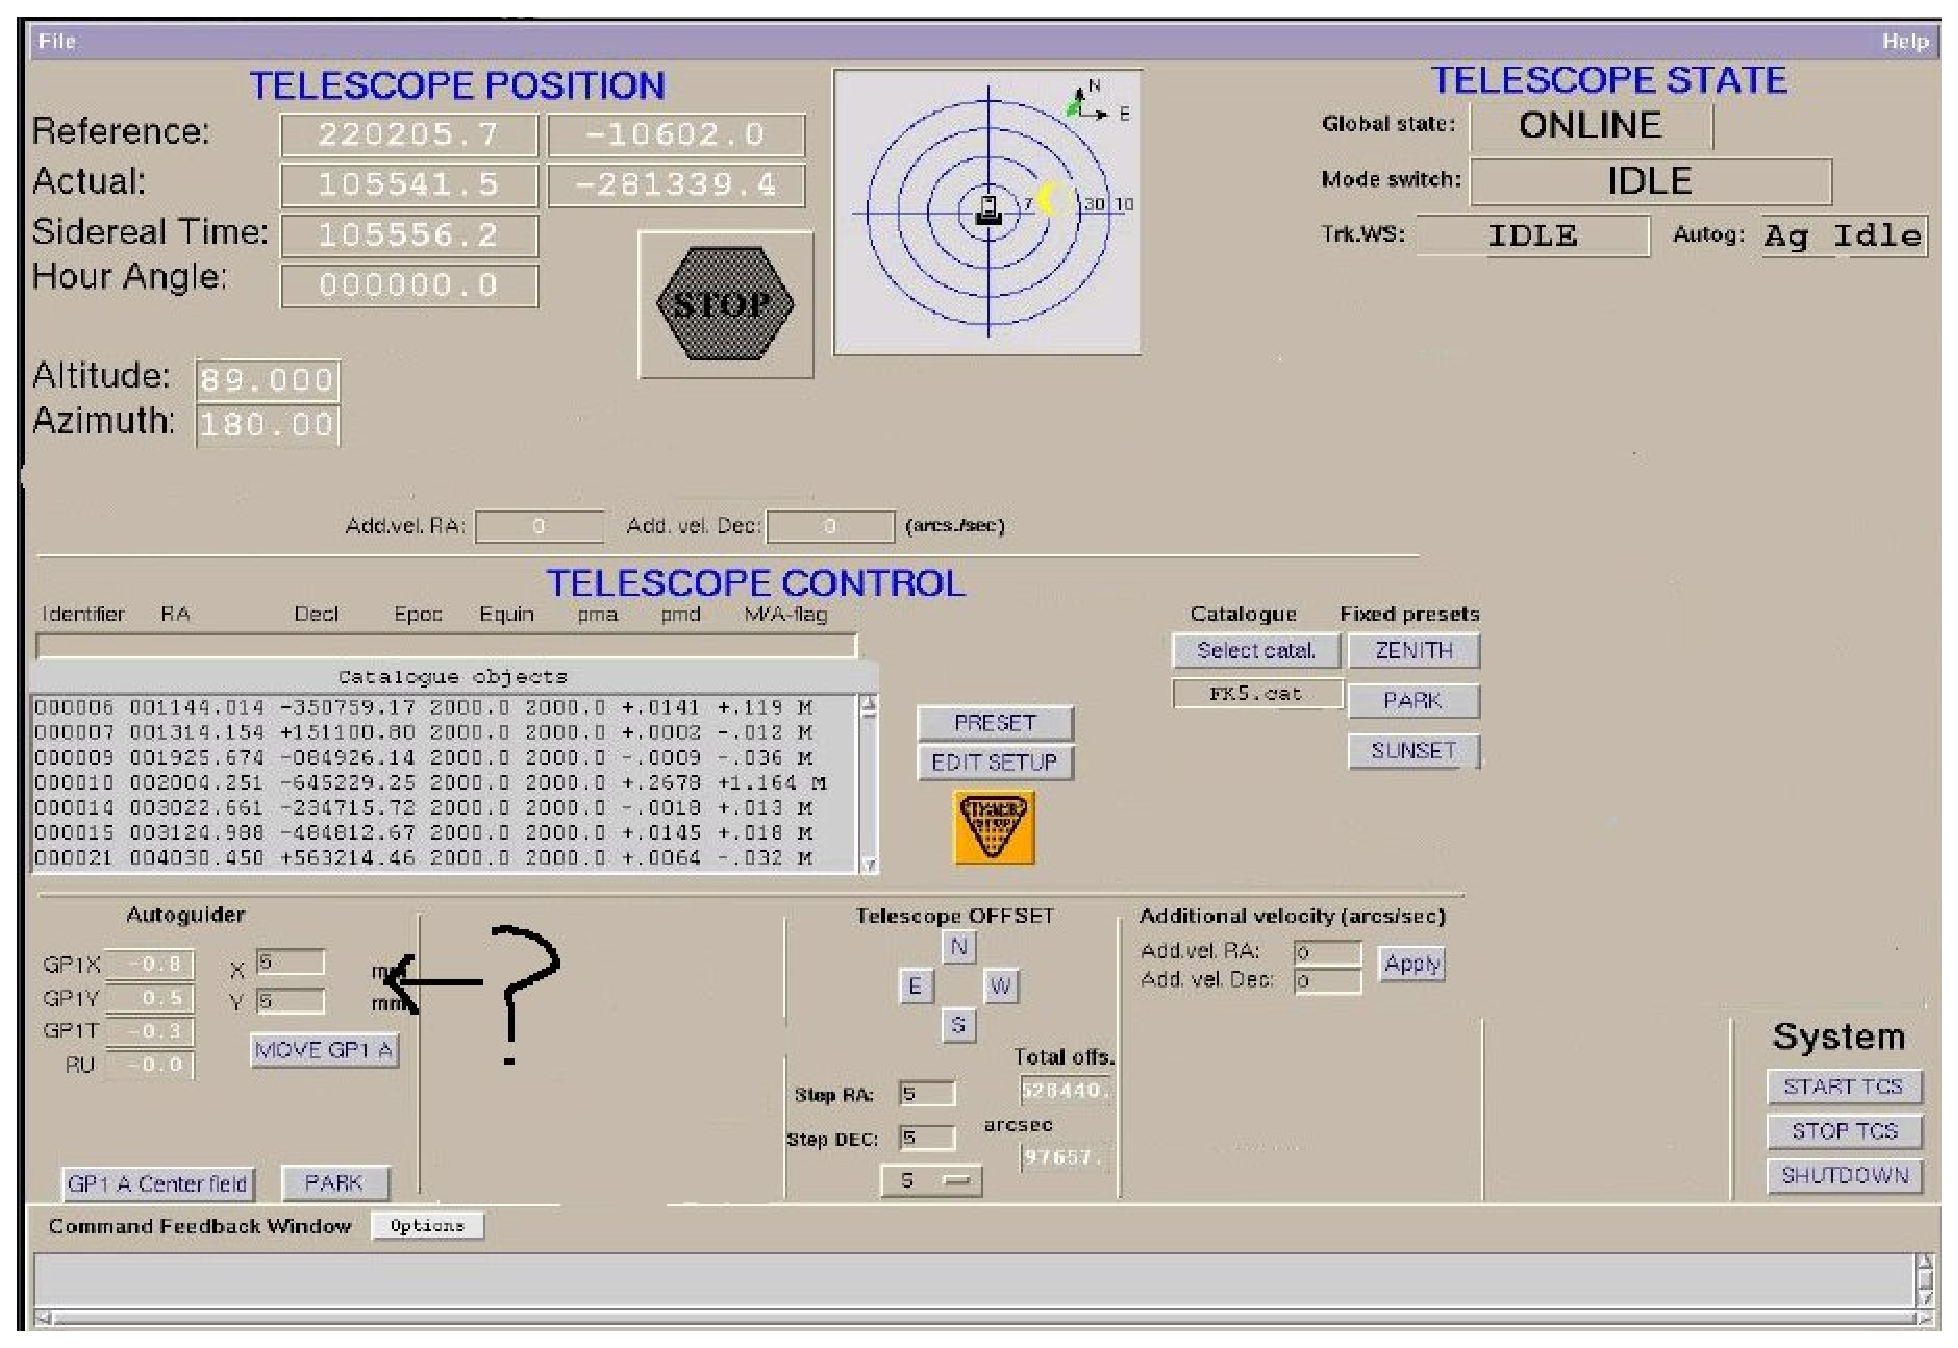
\includegraphics[scale=0.5]{tele.eps}
 \caption{Interfaz de un telescopio}
 %\label{fig:yeti}
\end{figure}


\newpage
\section{El Mercado}
%    *  �C�mo es el cliente real (superficie)?
%    * �A qu� segmento de mercado est� orientado?
%    * �Qu� posibilidades de evoluci�n de mercado existe (mercado potencial)?
%    * �Cu�l es el tama�o estimado? (Cuantificar).
%    * �Cu�l es mi competencia actual y potencial?
%    * Posibilidad del servicio como valor agregado.
%    * �De qu� forma se piensa penetrar, difundir en el mercado, mediante estrategias de marketing?

El cliente de Hevelius es un grupo de investigaci\'on astron\'omica que trabaja en el desarrollo de TCS 
(Sistemas de Control de Telescopios, por sus siglas en ingl\'es).
\\

Hevelius est\'a orientado a gente que trabaja con telescopios, ya sea en su proceso de operaci\'on o
en el estudio de las im\'agenes que el software provee.
\\

La gracia de Hevelius es que facilita el control de los telescopios, por lo que si la experiencia de 
nuestro cliente es exitosa, podemos tener a organizaciones completas (las cuales tienen diversos observatorios)
como futuros clientes y usuarios de nuestro software a nivel mundial.
\\

Si estimamos que un observatorio cuenta con un m\'inimo de 3 telescopios que usar\'an nuestro software 
y decimos que s\'olo en chile existen alrededor de 15 observatorios, son 45 unidades, vendibles, del software en Chile.
\\

Actualmente, no existe un software de las caracter\'isticas de Hevelius, por lo que no tenemos competencia 
en cuanto a la generalidad del uso del software. Sin embargo, el hecho de tener software creado espec\'ificamente
para cada telescopio es contar con una competencia fuerte que debe ser desplazada.

Existen reportes de que en Europa hay un grupo que desarrolla un software con el mismo fundamento que 
Hevelius, control gen\'erico de los telescopios, por lo que este futuro software ser\'a una competencia a tener
en cuenta.
\\

Para darle un valor agregado a nuestro producto, se puede ofrecer mantenci\'on y/o actualizaciones
de software a los clientes, lo que implica 2 l\'ineas de desarrollo: una que se dedica a corregir, mejorar 
el software comprado; y otra, que se dedica a crear una nueva versi\'on de Hevelius con nuevas caracter\'isticas
y que permite un nuevo negocio al ofrecer un software m\'as moderno y actualizado que el que se compr\'o.
\\

La mejor manera de entrar en el mercado cient\'fico-astron\'omico es demostrando con pruebas que el software
funciona realmente, por lo que es fundamental que nuestro cliente quede satisfecho con nuestro producto y as\'i 
se pueda usar esta experiencia como prueba fiel de \'exito. Sin embargo, no podemos dejar de lado una campa\~na



\newpage
\section{Precio del Producto}
%    *  �Cu�l es el costo real de los desarrolladores (horas de trabajo por tipo de trabajo)?
Para este Software se proyecta un tiempo de desarrollo de 1644 horas/hombre.
Cada hora/hombre posee un costo estimado de \$10.000, por lo que el costo de los desarrolladores es de
\$16.440.000 .


%    * �Cu�l es la inversi�n y cu�nto es la inversi�n en Hardware y Software necesario?
\begin{itemize}
\item Especificaciones del Software
La plataforma en la que se desarrolla actualmente Hevelius  consiste en el Sistema Operativo Linux, 
el software ACS 6.0, Java version "1.5.0\_04" y jogl-1\_0\_0-linux-i586.
Estos software todos de distribuci\.on gratuita, por lo que no hay un costo implicito en estos elementos
\item Especificaci\.on de Hardware
Los equipos con los cuales se desarrolla Hevelius poseen de las siguientes caracter�icas:
\begin{itemize}
\item 5 equipos: 4 para desarrollo, 1 para testing.
\item Procesador Pentium IV 3.0 Ghz de 32 bits.
\item 1Gb RAM
\end{itemize}
Con un costo de \$500.000 cada equipo y un costo total de \$2.500.000 .

Hardware externo ecesario para el desarrollo de Heveius:
\begin{itemize}
\item Telescopio NEXSTAR 4 SE que posee computador manual de 16 caracteres con pantalla LCD y 19 botones. 
Algunas de sus caracter�icas: apertura de 102 mm, largo focal de 1325 mm, radio focal de 12.99 mm, entre otras cosas.
Con un costo aproximado de \$500.000 .
\item Adjunto al telescopio una CCD para la obtenci\.on de im\.agenes. \$50.000 aproximados.
\item GPS para la obtenci\.on de ubicaci\.on de ubicaci\.on del telescopio. \$125.000 aproximados
\end{itemize}
\end{itemize}

%    * Identificar cu�les son los costos que existen antes de la puesta en marcha del producto. (arriendo, tel�fono, traslados, etc.).
Para este proyecto, se necesita tener durante 8 meses una oficina con espacio suficiente para 4-6 personas, 
5 equipos y 1 telescopio, por un valor cercano a los \$2.000.000. Adem\'as de lo anterior, es necesario contar 
con servicio telef\'onico a \$250.000 el periodo de desarrollo.

%    * Identificar cu�les son los costos de explotaci�n (de venta, mantenedores del producto, aparatos, etc.)
Para la obtenci\'on de los diversos componentes para el desarrollo de Hevelius, existen costos como el env\'io 
de Telescopio y CCD que tiene un costo de \$25.000, adem\'as de los costos de dise\~no del producto y publicidad 
de alrededor de \$100.000.
En lo referente a la oficina, la mantenci\'on de ella contratando una agencia de limpieza con un costo de \$100.000.
Para desarrollo tenemos contrato de Internet por los 8 meses que dure el proyecto \$320.000.

%    * Identificar cu�les son los impuestos y los gastos financieros que existen.
Los impuestos y gastos financieros asociados a Hevelius es \'unica y exclusivamente el I.V.A.

%    * Investigue y verifique cu�l es el precio actual de mercado de los productos similares.
En la actualidad, los software que existen y se venden tienen un valor cercano a los \$150.000 . No obstante, 
ciertos organismos astron\'omicos desarrollan sus propios software a un valor no informado.

%    * Determine cu�l es el precio estimado del producto (estimando n�mero de productos a vender y la utilidad esperada).

Estimamos que el software se puede vender a 5 organizaciones diferentes, por lo que ser\'ian 5 unidades, las cuales
se pueden vender a \$30.000.000 cada unidad. Con este precio obtenemos una utilidad de \$7.000.000 aproximadamente por unidad.



\newpage
\section{Los Emprendedores}
\subsection{Perfil de la empresa}

Nuestra empresa esta compuesta por cuatro alumnos de ingenier\'ia civil inform\'atica, dirigida hacia 
el desarrollo de diversos tipos de softwares. Para ello mencionamos la misi\'on y la visi\'on de nuestra empresa.

\subsubsection{Misi\'on}
Nuestra empresa pretende ser una ayuda a la ciencia, mediante el uso de la tecnolog\'ia inform\'atica en 
innovadores productos enfocados a diversas \'area del conocimiento.

\subsubsection{Visi\'on}
Nuestra visi\'on es trabajar mano a mano con los cient\'ificos e ingenieros del m\'as alto nivel, desarrollando 
software con altos est\'andares, el cual ser\'a usado y mantenido a lo largo del tiempo por la comunidad.

%    * Curr�culum de los integrantes (una p�gina cada uno).






\end{document}
